\subsection{Barrel and Forward Micromegas Trackers (BMT and FMT)}

\subsubsection{Geometry}

The Micromegas geometry is implemented through the native GEMC geometry API. There are two subsystems: a ``barrel'' micromegas
between the SVT and the CTOF, made by are three concentric regions divided azimuthally in three identical sectors; and a ``forward'' micromegas
made by three disk regions divided azimuthally in six identical sectors. In both subsystems each region is made by two layers,
one with wires parallel to the beam and one with wires perpendicular to the beam (see \F{bmtGeometry}).
Each micromegas sector contains a cover layer with copper ground, the printed circuit board (PCB) with the readout strips,
the Kapton support, the mesh layer, the ionizing gas, and other layers of material, listed in order below:

\begin{itemize}
	\item overlay
	\item copper ground
	\item PCB
	\item strips
	\item Kapton
	\item gas (amplification gap)
	\item mesh
	\item gas (drift detection gap)
	\item drift potential electrode
	\item foil
	\item ground
\end{itemize}

The sensitive volume contains argon/isobutane gas and is associated with the BMT and FMT hit process routines.
The geometry is summarized in \F{bmtGeometry}. The strip identification is performed in the Process ID routine.

\begin{figure}
	\centering
	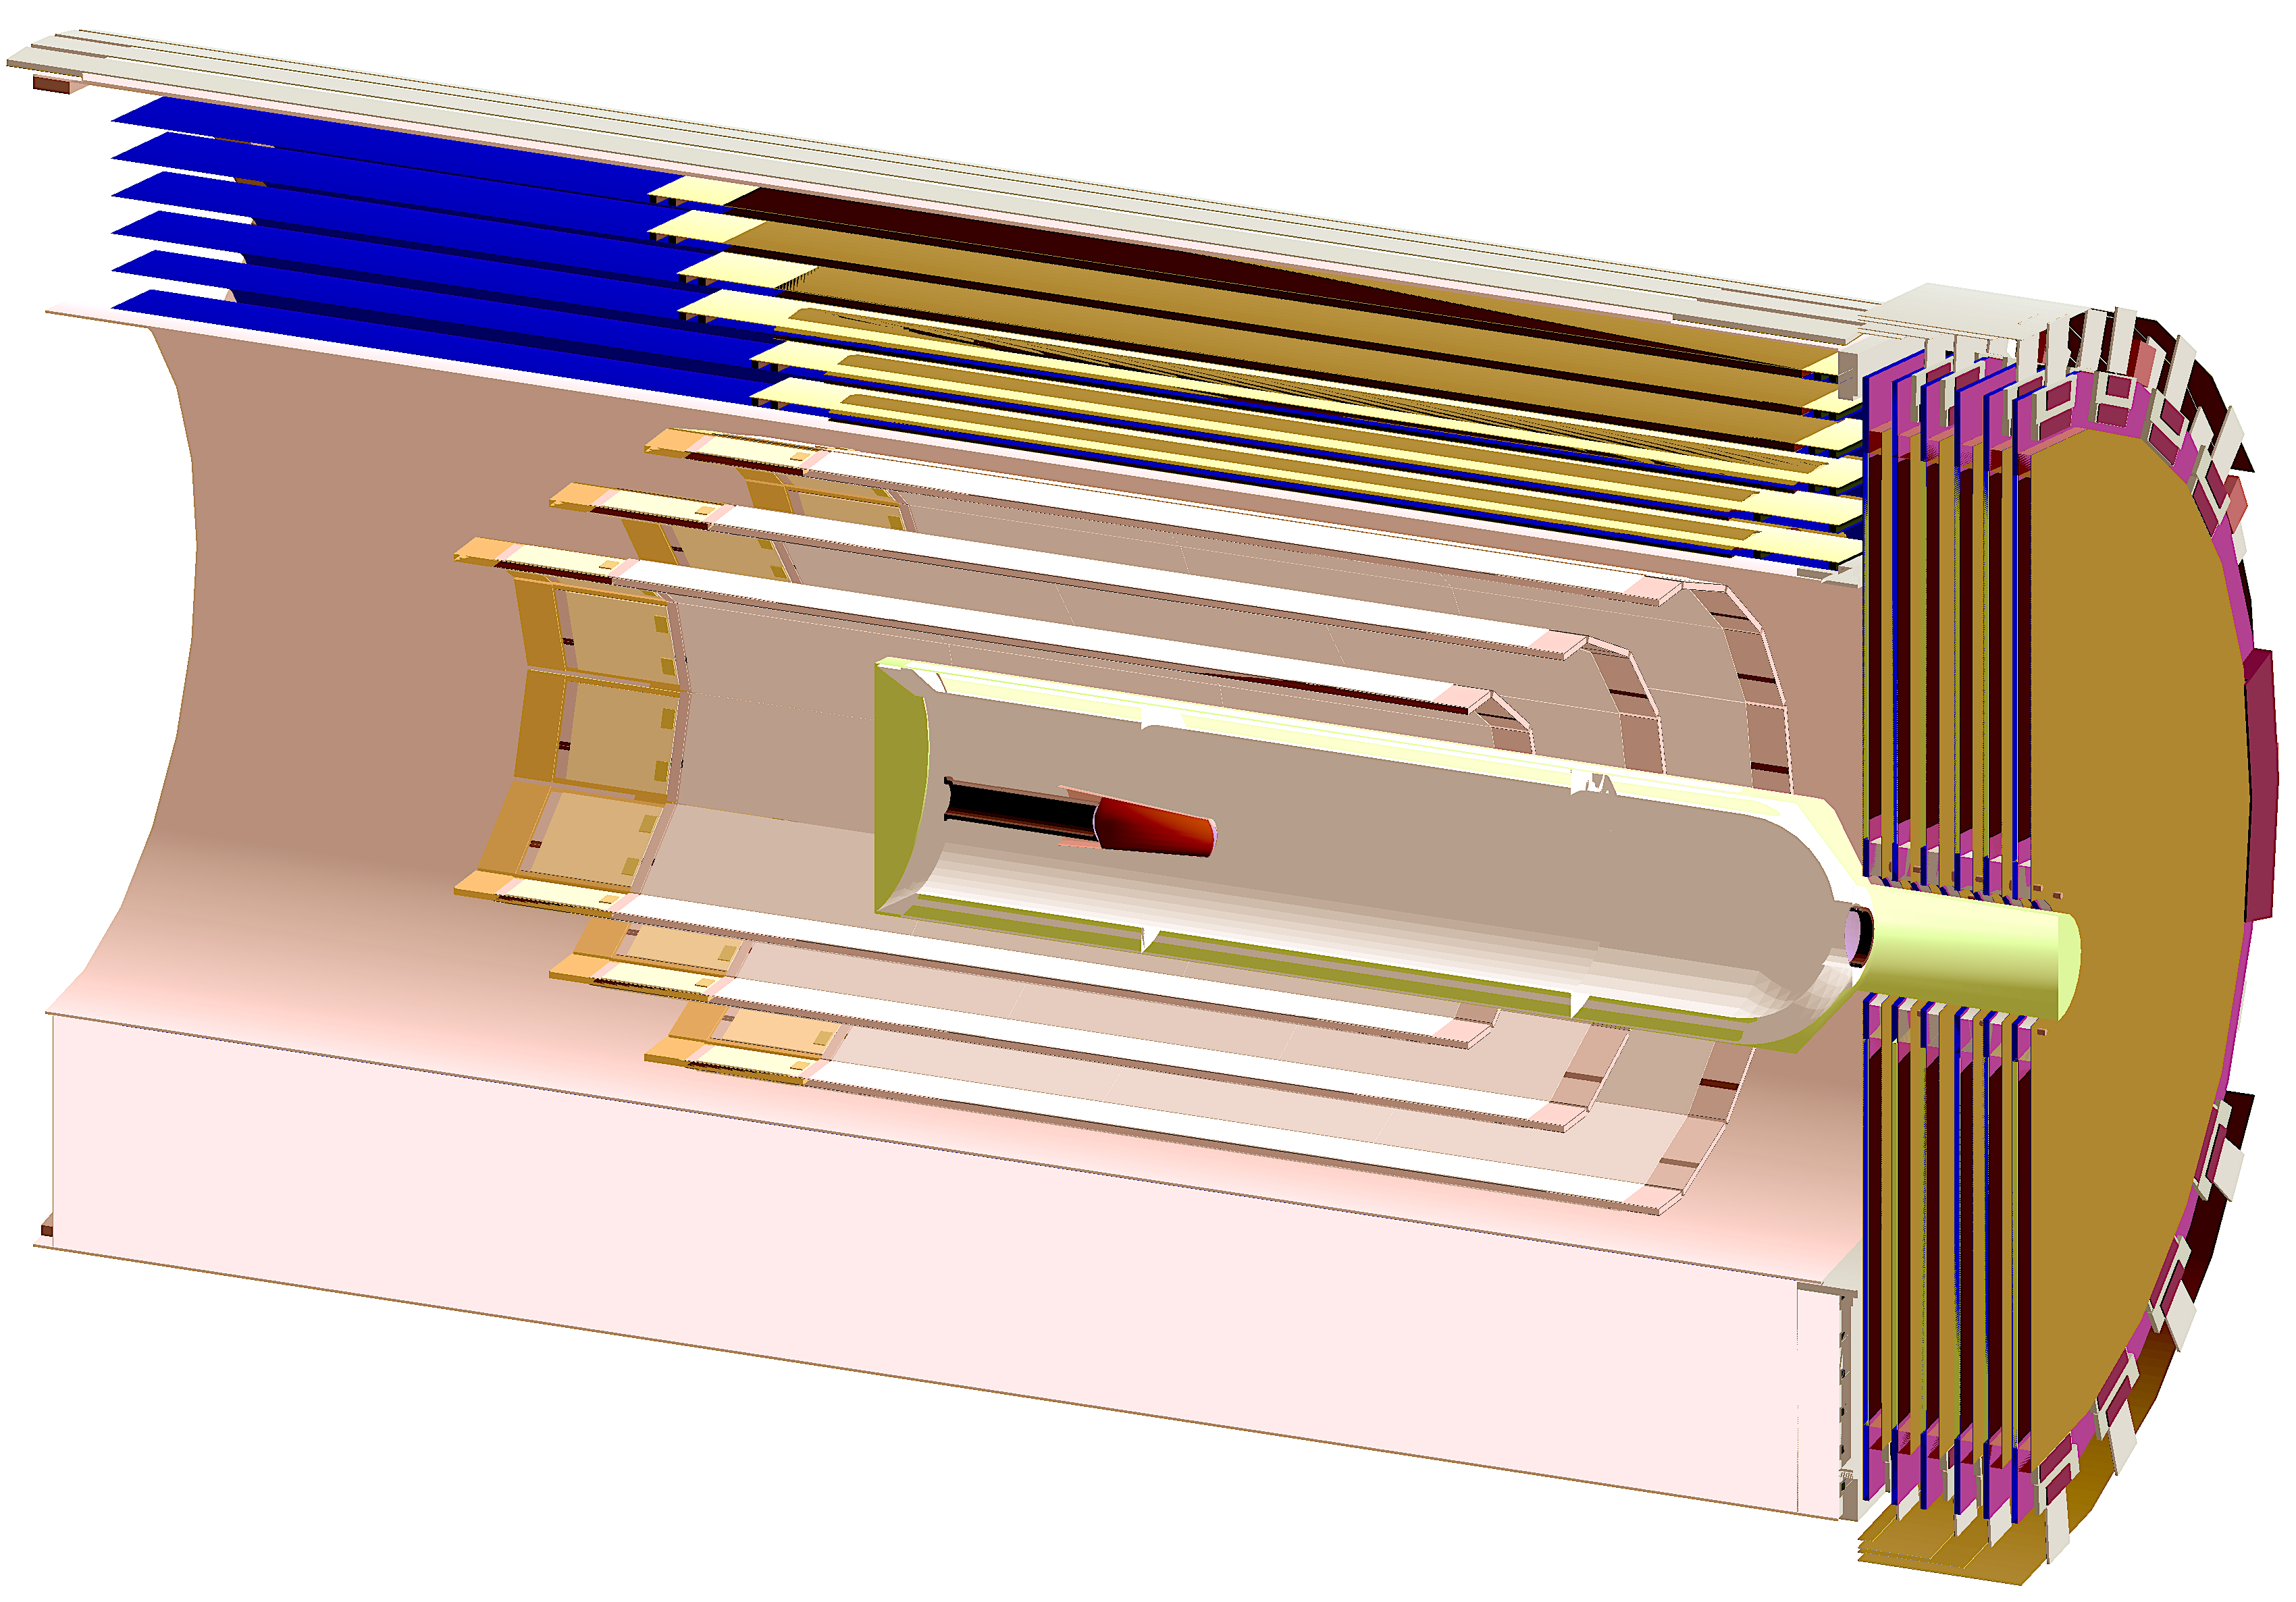
\includegraphics[width=0.99\columnwidth,keepaspectratio]{img/bmtGeometry.png}
	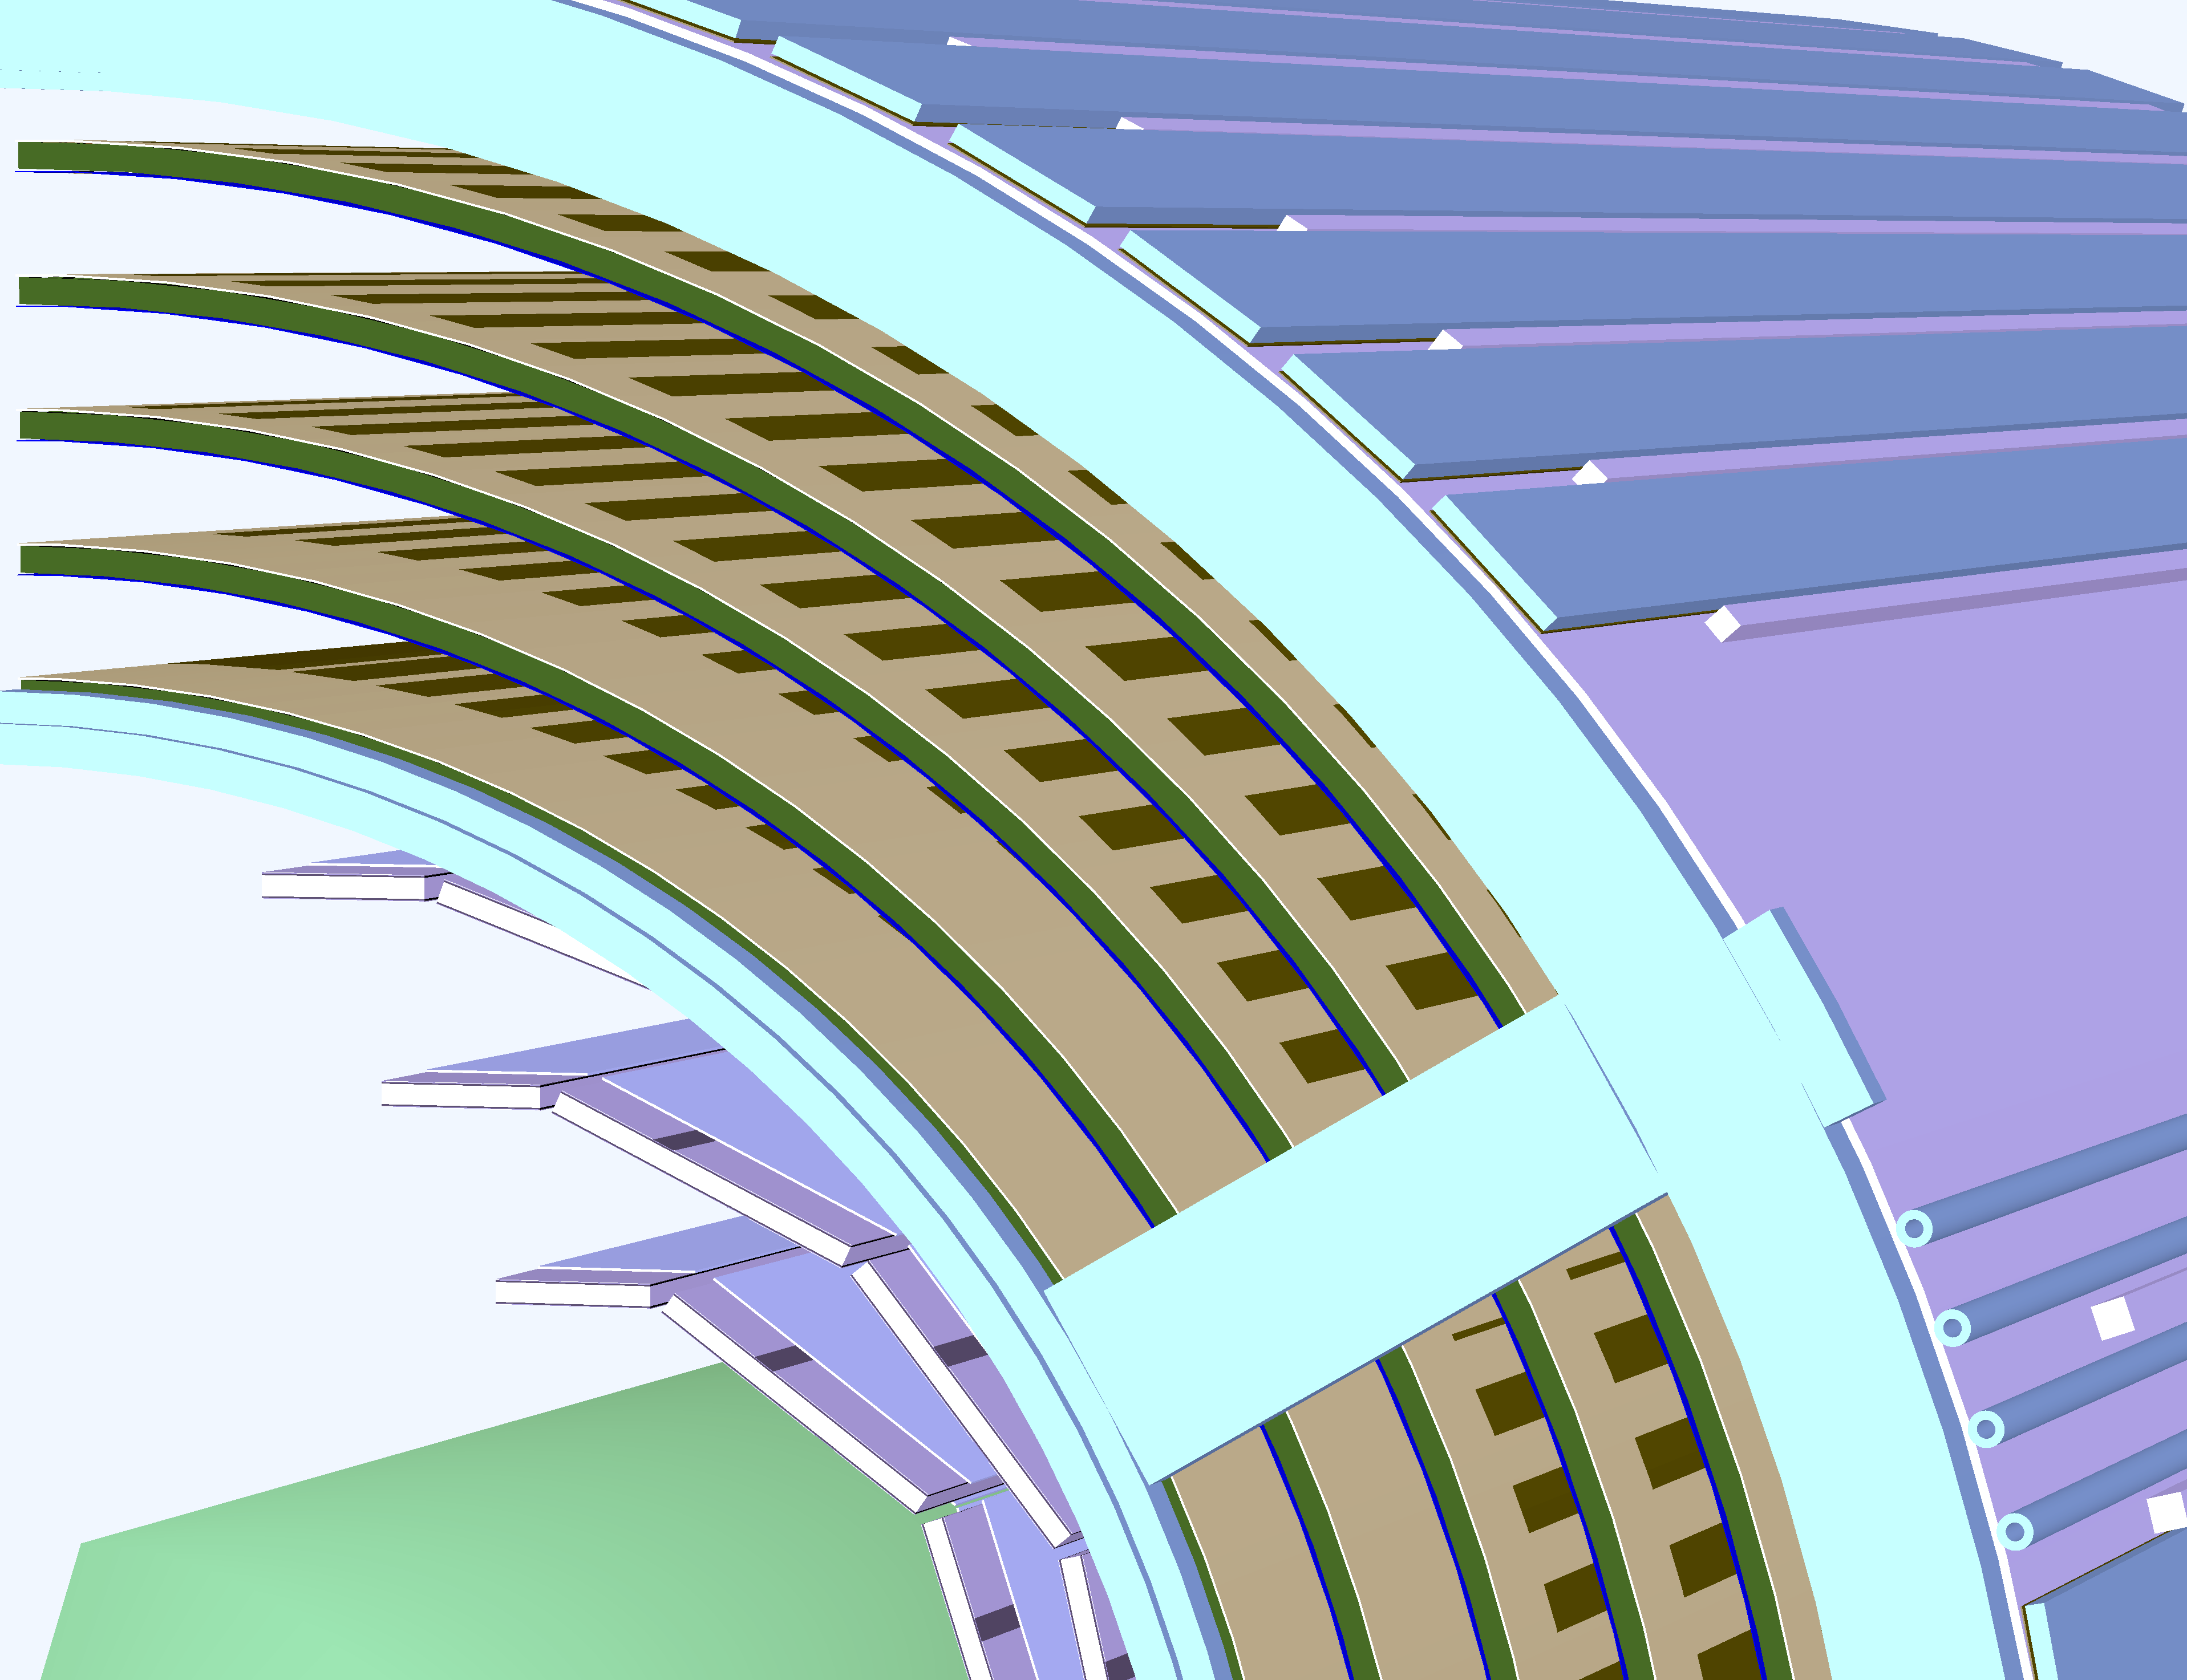
\includegraphics[width=0.99\columnwidth,keepaspectratio]{img/bmtDetail.png}
	\caption{Top: a longitudinal cut view ($x>0$ only) of the CLAS12 Central Detector trackers. The target is surrounded by 3 layers of SVT and
            6 layers of micromegas, 3 with $z$-strips, 3 with $c$-strips. On the downstream end (beam incident from the left)
			the Forward Micromegas Tracker disks are visible.
            Bottom: detail of the micromegas GEMC geometry, showing the overlay cover, the copper ground, and the PCB.}
	\label{fig:bmtGeometry}
\end{figure}


\subsubsection{Process ID}
At each Geant4 step, the local coordinates in the sensor volume are used to calculate the strip number.
The algorithm includes the Lorentz angle based on the magnetic field strength, the particle direction,
the pitch angle between the strips, and the dead zones of the sensitive parts.
A virtual electron avalanche is simulated based on the energy deposited. The avalanche
is deposited onto one strip or distributed among several to account for the energy sharing.



\subsubsection{Digitization}

The Micromegas digitization provides the ADC value calculated using the total energy deposited (after hit sharing).
There is no timing information in the output.
The digitized output bank variables are summarized in Table \ref{tab:mmBank}.

\begin{table}[h]
	\begin{center}
		\begin{tabular}{| c | c | c |}
			\hline \hline
			Variable & Description  \\
			\hline
              layer  &      layer number   \\
             sector  &     sector number   \\
              strip  &      strip number   \\
               Edep  &  energy deposited   \\
                ADC  &               ADC   \\
			\hline \hline
		\end{tabular}
	\end{center}
	\caption{The digitized BMT and FMT banks.}\label{tab:mmBank}
\end{table}

The time window  of the Micromegas is set to to 132 ns: all Geant4 steps within the same strip and time window are collected in one hit.

